\section{Parámetros de la ecuación de estado cúbica}\label{sec:parameters}

El cálculo de los parámetros depende de la cantidad de compuestos presentes en el sistema.

\begin{itemize}
 \item Para los compuestos puros la clase `Substance' define el cálculo de los parámetros usando una expresión de $\alpha$ , los parámetros $\Omega_a$ y $\Omega_b$ de la ecuación de estado y las propiedades del compuesto puro.
 \item Para las mezclas, la clase `Mixture' define el cálculo de los parámetros usando una regla de mezclado y el cojunto de los parámetros  $a$ y $b$ calculados a partir de los compuestos puros.
\end{itemize}


Esta estructura se muestra en laf figura \ref{fig:homogeneousCalculations}

\begin{figure}[!h]
  
  \centering
    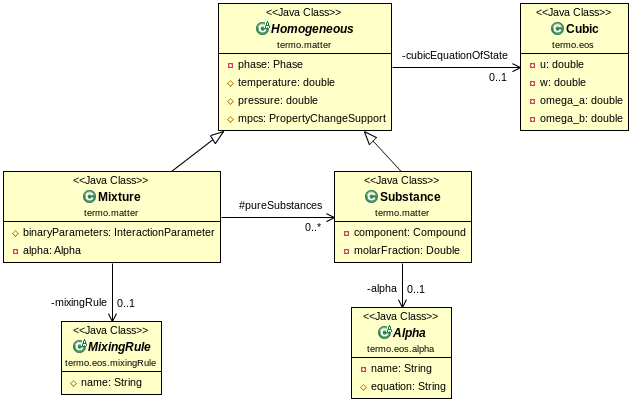
\includegraphics[scale=0.7]{homogeneousCalculations.png}
    \caption{Estructura de la librería para el cálculo de propiedades.}
    \label{fig:homogeneousCalculations}
\end{figure}

Nótese de la figura \ref{fig:homogeneousCalculations} los siguiente:
\begin{itemize}
	\item Que la clase `Homogeneous' contiene una ecuación del tipo `Cubic'.
 	\item Que las clases `Substance' y `Mixture' heredan las propiedades de la clase `Homogenous', como la ecuación cúbica, y puede hacer uso de ella.

\end{itemize}

	Cualquiera de las dos implementaciones de la clase `Homogeneous' tiene los métodos necesarios para calcular los parámetros de la ecuación cúbica según el código \ref{lst:homogeneousParameters}.

\begin{lstlisting}[caption=Cualquier objeto tipo `Homogeneous' puede calcular los parámetros de la ecuación de estado cúbica a y b, label={lst:homogeneousParameters}]
	Homogeneous homogeneous = ...// Objeto tipo `Homogeneous'.
	double a = homogeneous.calculate_a_cubicParameter();
	double b = homogeneous.calculate_b_cubicParameter();
\end{lstlisting}


\subsection{Compuesto puro}\label{subsec:substance}

Como se muestra en la figura \ref{fig:homogeneousCalculations} la clase `Substance' continene una expresión de $\alpha$, y una ecuación de estado, necesarias para realizar el cáculo de los parámetros, segun las ecuaciones \ref{eq:a} y \ref{eq:b}. 

La expresión de $\alpha$ puede ser una función de la temperatura, las expresiones implementadas en el presente trabajo se muestran en la tabla \ref{tab:alphas}.

\begin{table}[!h]
	\centering
	\caption{Expresiónes de $\alpha$ disponibles en la librería}\label{tab:alphas}
	\begin{tabular}{|c|c|c| }
		\hline
		Expresión & Parámetros & Ecuación de estado\\
		\hline
		Soave    &  ---& PR\\
		Peng and Robinson & ---& PR \\
		Mathias & $A$ & SRK\\
		Stryjek and Vera & $k_1$ & PRSV\\
		Adachi and Lu & $A,B$&SRK,PR\\
		Soave & $A,B$&SRK,PR\\
		Melhem, et al. & $A,B$&SRK,PR\\
		Androulakis et al. & $A,B,C$& SRK,PR\\
		Mathias and Copeman & $A,B,C$& SRK,PR\\
		Yu and Lu & $A,B,C$&SRK,PR\\
		Stryjek and Vera & $A,B,C$&PR\\
		Twu & $L,M,N$&TST\\
		Twu & ---&TST,PR\\
		GCEOS & ---& (Cualquier u y w)\\
		\hline
	\end{tabular}
\end{table}
\subsubsection{Creación de un objeto tipo `Substance'}\label{subsub:substanceCreation}

Es necesario utilizar el método constructor de la clase `Substance' para crear un objeto de este tipo, se debe proporcionar como parámetros la ecuación de estado deseada, la exprsión de $\alpha$, una instancia de la clase `Compound' como se muestra en la sección \ref{sec:compounds} y la fase de la substancia.

En la sección \ref{subsec:cubicCreation} se mostró como crear una ecuación de estado cúbica previamente definida, a través de la clase `EquatiosOfState'. Los valore de $\Omega_a$ y $\Omega_b$ se muestran en la tabla \ref{tab:cubics}. De forma muy similar al de las ecuaciońes de estado,la selección de la expresión de $\alpha$ se realiza a través de la clase `Alphas'.

El código \ref{lst:substanceCreation} muestra como crear una objeto del tipo substancia.

\begin{lstlisting}[caption={Creación de un objeto tipo `Substance' para el compuesto Ciclohexano, con la ecuación de estado Soave Redlich Kwong y la expresión de $\alpha$ de mathias },label={lst:substanceCreation}]

Compound compound = new Compound("Cyclohexane");
compound.setCriticalPressure(4073000);
compound.setCriticalTemperature(553.5);
compound.setAcentricFactor(0.211);


Cubic srk = EquationsOfState.redlichKwongSoave();
Alpha mathias = Alphas.getMathiasExpression();


Substance substance = new Substance(srk,mathias, compound,Phase.LIQUID);
\end{lstlisting}

	Finalmente se utiliza el objeto creado para realizar el cálculo de los parámetros de la ecuación de estado cúbica, en el código \ref{lst:substanceParams}.

\begin{lstlisting}[caption={Cálculo de los parámetros para la ecuación de estado cúbica con la clase `Substance'.},label={lst:substanceParams}]
double a = substance.calculate_a_cubicParameter();
double b = substance.calculate_b_cubicParameter();
\end{lstlisting}
 

Nótese que el código \ref{lst:homogeneousParameters} y el código \ref{lst:substanceParams} es idéntico y aunque parece redundate, solo se muestra para señalar el polimorfismo de la librería , es decir que el objeto substance es del tipo `Homogeneous' además del tipo `Substance', y tiene accesso a los métodos en las dos clases.


\subsubsection{Mezcla}\label{subsec:mixture}

El cálculo de los parámetros para una mezcla depende de la regla de mezclado, y en el caso de las reglas de mezclado basadas en la energía libre de exceso, también del modelo de actividad.

Las reglas de mezclado incluidas en este trabajo se muestran en la tabla \ref{tab:mixingrules}, y los modelos de actividad se listan en la tabla \ref{tab:activitymodels}.

\begin{table}[!h]
	\caption{Reglas de mezclado implementadas}\label{tab:mixingrules}
	\begin{tabularx}{\textwidth}{|X|X|X|}
		\hline
		Regla & Parámetros & \\
		\hline
		Van Der Waals & $k_{ij}$ & $k_{ij} = k_{ji}$ \\
		Mathias-Klotz-Prausnitz& $k_{ij}$ & $k_{ij} \neq k_{ji}$ \\
		Huron Vidal & Según el model de actividad & \\
		Wong Sandler & $k_{ij}$ + los parámetros del modelo de actividad & $k_{ij} = k_{ji}$ \\
		\hline
	\end{tabularx}
\end{table}

\begin{table}[!h]
	\caption{Modelos de actividad }\label{tab:activitymodels}
	\begin{tabularx}{\textwidth}{|X|X|X|}
		\hline
		Modelo de actividad & Parámetros & \\
		\hline
		Wilson & $a_{ij}$, $b_{ij}$  & \\
		NRTL & $a_{ij}$, $b_{ij}$, $\alpha_{ij}$ & $\alpha_{ij} = \alpha_{ji}$ \\
		\hline
	\end{tabularx}
\end{table}
\subsubsection{Creación de un objeto tipo `Mixture'}\label{subsub:mixtureCreation}

Un objeto tipo `Mixture' contiene dentro de sí un conjuto de objetos tipo `Substance', esto hace que su creación sea mas compleja. Se ha escrito la clase `MixtureBuilder' para facilitar la creación de los objetos de la clase `Mixture'.

La clase `MixtureBuilder' facilita la creación de los objetos `Substance' que forman el conjunto de compuestos de la mezcla, y permite asignar una expresión de $\alpha$ diferente para cada compuesto.

El código \ref{lst:mixturecreation} muestra la creación de una mezcla, donde la expresión de $\alpha$ es la misma para cada compuesto puro. 

\begin{lstlisting}[caption={Creación de una mezcla con la clase `MixtureBuilder' asignando la misma expresión de $\alpha$ para cada compuesto puro.}, label={lst:mixturecreation} ]

Compound cyclohexane = new Compound("Cyclohexane");
cyclohexane.setCriticalPressure(4073000);
cyclohexane.setCriticalTemperature(553.5);
cyclohexane.setAcentricFactor(0.211);

Compound pentane = new Compound("N-pentane");
pentane.setCriticalPressure(3370000);
pentane.setCriticalTemperature(469.7);
pentane.setAcentricFactor(0.251);

Cubic equationOfState = EquationsOfState.pengRobinson();
Alpha alpha = Alphas.getMathiasAndCopemanExpression();

Mixture mixture = new MixtureBuilder()
			.addCompounds(cyclohexane,pentane)
			.setAlpha(alpha)
			.setEquationOfState(equationOfState)
			.setPhase(Phase.VAPOR)
			.build();

\end{lstlisting}

Es posible crear la mezcla con una expresión de $\alpha$ diferente para cada compuesto puro según el código \ref{lst:mixtureParametersDifAlphas}. 


\begin{lstlisting}[caption={Código para el cálculo de los parámetros de la ecuación de estado en una mezcla, con diferentes expresiones de $\alpha$},label={lst:mixtureParametersDifAlphas}]
Mixture mixture = new MixtureBuilder()
			.addCompound(cyclohexane,Alphas.getPengAndRobinsonExpression())
			.addCompound(pentane,Alphas.getStryjekAndVeraExpression())
			.setEquationOfState(eos)
			.setPhase(phase)
			.setMixingRule(mixingRule)
			.setInteractionParameter(k)
			.build();
\end{lstlisting}

Finalmente se pueden calcular los parámetros de la ecuación cúbica con el código \ref{lst:mixtureParameters}.

\begin{lstlisting}[caption={Cálculo de parámetros de la mezcla},label={lst:mixtureParameters}]
double a = mixture.calculate_a_cubicParameter();
double b = mixture.calculate_b_cubicParameter();
\end{lstlisting}
